\documentclass[border=8pt]{standalone}
\usepackage[T1]{fontenc}
\usepackage{tgpagella}
\usepackage{amsmath}
\usepackage{tikz}
\usetikzlibrary{arrows.meta,positioning,fit,backgrounds}

\definecolor{ink}{HTML}{16140F}
\definecolor{mid}{HTML}{5C5849}
\definecolor{light}{HTML}{D9D6C8}
\definecolor{navy}{HTML}{2E5B88}
\definecolor{navybg}{HTML}{EBF1F6}
\definecolor{ochre}{HTML}{B86B28}
\definecolor{ochrebg}{HTML}{FAF2EA}
\definecolor{paper}{HTML}{F7F5EE}

\tikzset{
  blk/.style={draw=ink,line width=0.6pt,rounded corners=2pt,fill=white,font=\small,align=center,inner sep=5pt},
  blkg/.style={blk,fill=paper},
  blkn/.style={blk,fill=navy!18},
  blko/.style={blk,fill=ochre!22},
  arr/.style={-{Stealth[length=2.2mm]},line width=0.6pt,draw=ink},
  lbl/.style={font=\scriptsize\itshape,text=mid},
  st/.style={blk,minimum width=92mm,minimum height=9.5mm,text width=88mm,align=left},
  grpblue/.style={draw=navy,dashed,line width=0.7pt,rounded corners=4pt,fill=navybg,fill opacity=0.45,inner sep=7pt},
  grpochre/.style={draw=ochre,dashed,line width=0.7pt,rounded corners=4pt,fill=ochrebg,fill opacity=0.55,inner sep=7pt},
}

\begin{document}
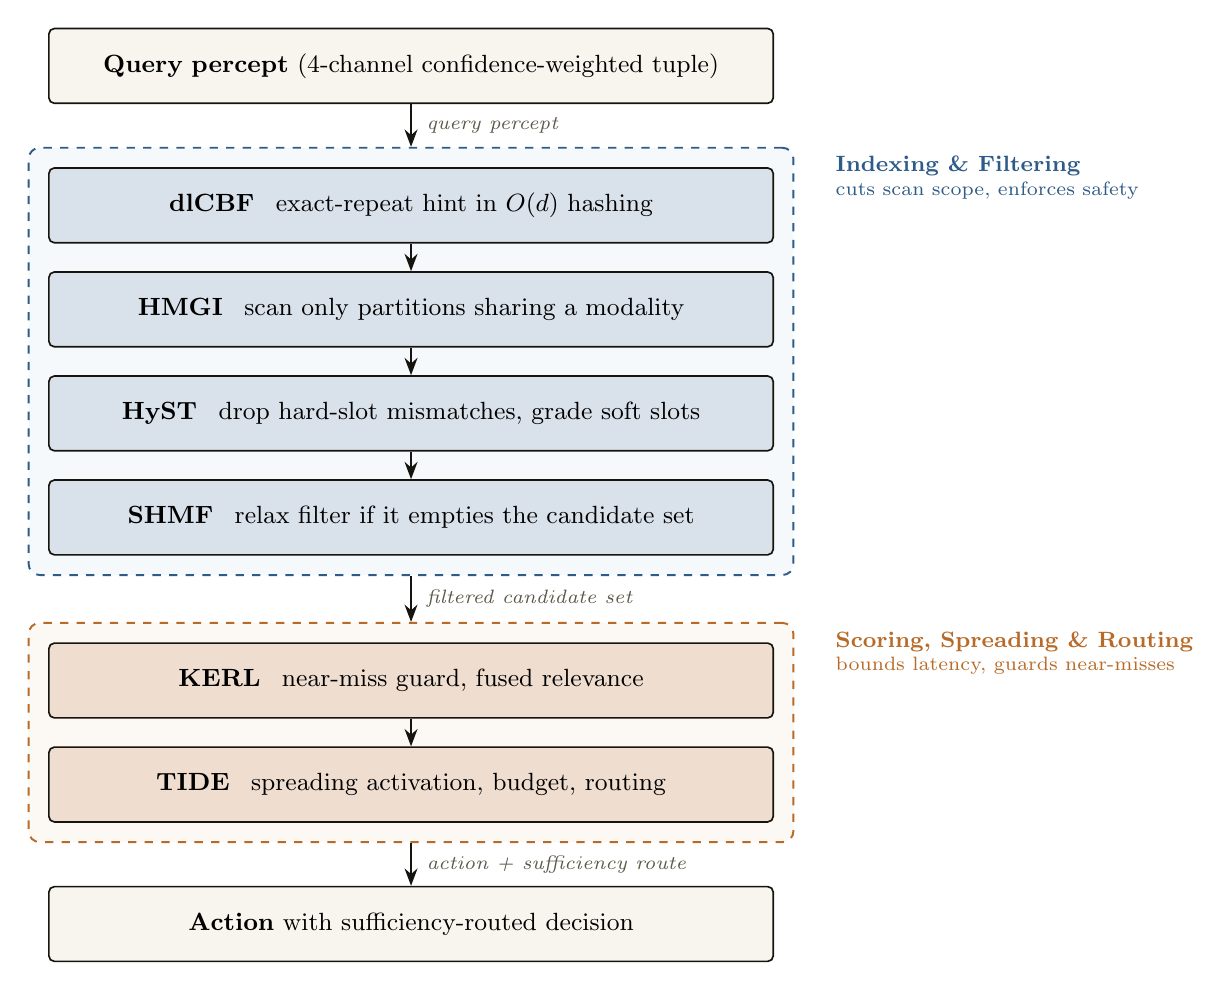
\begin{tikzpicture}[node distance=3.5mm]
  % Input
  \node[st,blkg] (q) {\textbf{Query percept} (4-channel confidence-weighted tuple)};

  % Blue section nodes
  \node[st,blkn,below=8mm of q] (c1) {\textbf{dlCBF} \enspace exact-repeat hint in $O(d)$ hashing};
  \node[st,blkn,below=of c1] (c2) {\textbf{HMGI} \enspace scan only partitions sharing a modality};
  \node[st,blkn,below=of c2] (c3) {\textbf{HyST} \enspace drop hard-slot mismatches, grade soft slots};
  \node[st,blkn,below=of c3] (c4) {\textbf{SHMF} \enspace relax filter if it empties the candidate set};

  % Brown/Ochre section nodes
  \node[st,blko,below=11mm of c4] (c5) {\textbf{KERL} \enspace near-miss guard, fused relevance};
  \node[st,blko,below=of c5] (c6) {\textbf{TIDE} \enspace spreading activation, budget, routing};

  % Output
  \node[st,blkg,below=8mm of c6] (out) {\textbf{Action} with sufficiency-routed decision};

  % Group boxes on background layer
  \begin{scope}[on background layer]
    \node[grpblue,fit=(c1)(c2)(c3)(c4)] (gblue) {};
    \node[grpochre,fit=(c5)(c6)] (gochre) {};
  \end{scope}

  % Section headers on right
  \node[right=4mm of gblue.north east,anchor=north west,font=\footnotesize\bfseries,text=navy,align=left] {Indexing \& Filtering\\[-1pt]\scriptsize\itshape\normalfont cuts scan scope, enforces safety};
  \node[right=4mm of gochre.north east,anchor=north west,font=\footnotesize\bfseries,text=ochre,align=left] {Scoring, Spreading \& Routing\\[-1pt]\scriptsize\itshape\normalfont bounds latency, guards near-misses};

  % Internal arrows
  \draw[arr] (c1) -- (c2);
  \draw[arr] (c2) -- (c3);
  \draw[arr] (c3) -- (c4);
  \draw[arr] (c5) -- (c6);

  % Section I/O arrows
  \draw[arr] (q.south) -- node[lbl,right=2pt]{query percept} (gblue.north);
  \draw[arr] (gblue.south) -- node[lbl,right=2pt]{filtered candidate set} (gochre.north);
  \draw[arr] (gochre.south) -- node[lbl,right=2pt]{action + sufficiency route} (out.north);
\end{tikzpicture}
\end{document}
